\documentclass{article}
% these are packages - graphicx allows for including pictures, fullpage makes sane margins, and hyperref allows inclusion of urls.
\usepackage{graphicx,fullpage,hyperref}

% comments are prefaced by the percentage sign
%
%

\title{MTH 765P Mini-project}
\author{Your name here}
\date{}

% NOTE
%----------------
% you do not need to follow this format -- this is just a suggestion!
%

\begin{document}
\maketitle
% You do not need an abstract
\section{Introduction}
Here is where you introduce the dataset - what is it, where did you get it, etc. Here we will also see how to refer to figures, see Figure~\ref{figure1}.

\begin{figure}[htbp]
    % you can specify height or width of an image
    % do not forget to specify a unique name for each image and make sure all figures have a caption
    % the
    \centering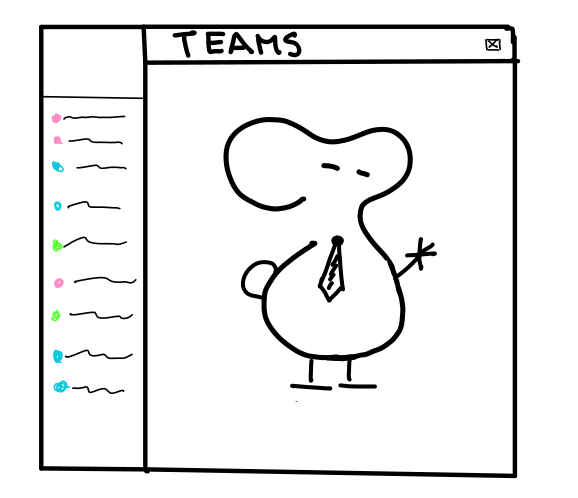
\includegraphics[width=0.5\textwidth]{teams.png}
    \caption{\label{figure1} This is a figure.}
 \end{figure}

 \section{Obtaining/Acquiring the Data}
 How did you get it? What did you need to do?


 \section{Description}
 More in detail than in the introduction -- Here is a web address \url{www.arxiv.org}.
 
 \section{Analysis}
Presentation of some aspects of the data (including visualisations)

Make sure to point out which libraries you used.

\section{Questions}
What would you do if you had to do more analysis on the dataset? Do you need additional data? Are there interesting questions that one could try to answer? 
Consider what would you do if this was a more in-depth project. Note here you should just think about possible directions (you do not need to follow up or 
justify them).

\end{document}